\documentclass[10.5pt]{article}
\usepackage{xeCJK}%preamble part
\usepackage{graphicx}
\usepackage{indentfirst}
\usepackage[a4paper, inner=1.5cm, outer=3cm, top=2cm, bottom=3cm, bindingoffset=1cm]{geometry}
\usepackage{epstopdf}
\usepackage{array}
\usepackage{fontspec}
\usepackage{gensymb}
\usepackage[lofdepth,lotdepth]{subfig}
\setCJKmainfont[BoldFont={SimHei}]{SimSun}
\setCJKmonofont{SimSun}
\setmainfont{Times New Roman}
\newCJKfontfamily[hei]\heiti{SimHei}
\setlength{\extrarowheight}{4pt}
\begin{document}
\title{\textbf{\fontsize{15.75pt}{\baselineskip}{界面法测定电解反应氢离子迁移速率实验报告}}} % 15.75pt is 3 号 in chinese
\author{\fontsize{12pt}{\baselineskip}{数33 赵丰 2013012178 \quad }}
\maketitle
\section{\textbf{\fontsize{12pt}{\baselineskip}{引言}}}
本次实验用界面法测定乙酸乙酯皂化反应速率常数,在电解反应中,电解液中的阴阳离子分别向阳极和阴极移动,转移的电子数等于阴阳离子迁移数的总和,一般阴阳离子的贡献是不相等的,对电解0.1mol/L的盐酸溶液反应来说,$H^+$的迁移率约在80\%左右。\\
测定$H^+$迁移率即需要知道一段时间内通过导电回路总的电荷量和在阴极得电子的$H_2$总量。总的电荷量可通过万用电表的电流值对时间做数值积分得到,阴极得电子的$H_2$总量可通过界面法测量。\\
对本实验来说,采用镉电极作阳极,用甲基橙作指示剂,盐酸溶液显橙红色,而被电解的镉离子近似无色,溶液中失去的$H^+$离子由镉离子补充,这样随着反应的进行,反应导管中的无色液柱逐渐上升,通过记录一段时间液柱上升的体积,并假设阳离子浓度基本不变根据电荷守恒,可得该段时间内$H^+$迁移量为$Q=FV*0.1mol/L$,其中F=96485C/mol,为Faraday常数。
\section{\textbf{\fontsize{12pt}{\baselineskip}{实验操作}}}

\subsection{\textbf{\fontsize{12pt}{\baselineskip}{实验操作步骤及方法要点}}}
本次实验使用多路直流稳定电源,可以分别做稳压源和稳流源使用,为实验分别在恒压(6~7V)和恒流(3A左右)提供了条件。
无论是恒压条件还是恒流条件,每次测量步骤大致如下
\begin{enumerate}
\item 用助教配得的盐酸溶液的浓度为0.0961mol/L,对反应导管进行润洗。
\item 用超级恒温水浴装置对反应导管进行恒温(25\degree C),接好电路后(银电极为负极,镉电极为正极),待无色液面上升至反应导管零刻度线后打开秒表开始记录数据,反应持续时间大约20分钟。
\item 反应结束后,将废液倒入回收桶中。
\end{enumerate}
\section{\textbf{\fontsize{12pt}{\baselineskip}{结果与讨论}}}
\subsection{\textbf{\fontsize{12pt}{\baselineskip}{原始实验数据}}}
将万用表和秒表记录的数据作图如下:
\begin{figure}[!ht]
\centering
\caption{恒压条件导电回路电流随时间变化曲线}
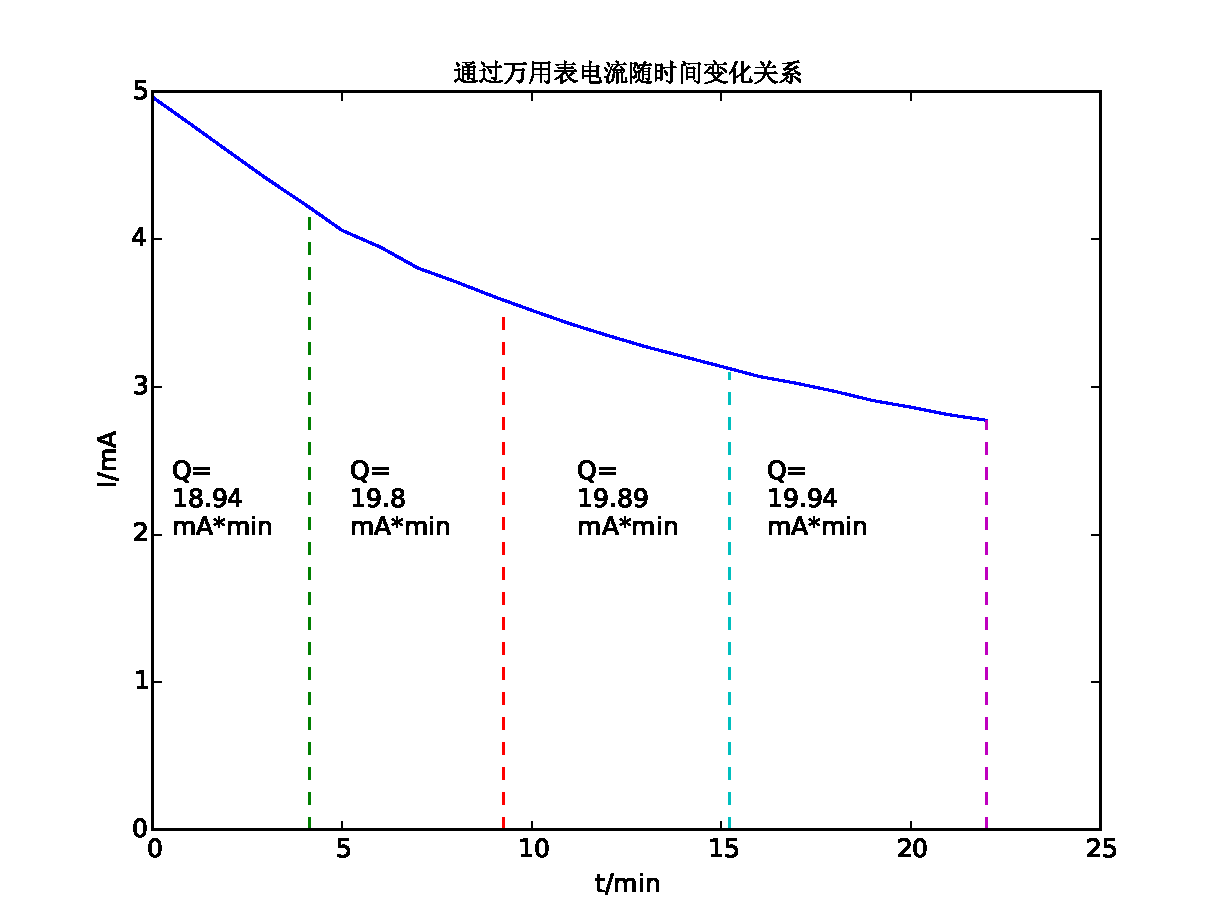
\includegraphics[width=400pt]{pc_2.pdf}
\end{figure}
可见,随着反应的进行,阳极镉离子浓度增加以及阴极氢离子浓度减少,都使得反应速率下降。
上图中4条虚线分别表示界面上升到0.1,0.2,0.3和0.4mL时对应的时间,其中在每个区域的文本框中标明了该0.1mL的液体对应的曲边梯形的面积,由于第一个面积的计算值与后面三个相差较大,故只对后三个取平均值,再代入公式,最后算得氢离子的迁移率为0.78.
利用恒流法(I为22.944mA左右)得到的实验数据如下表所示:
\begin{table}[!ht]
\centering
\caption{恒流法实验结果}
\begin{tabular}{cccccc}
\hline
时间(min) & 0 & 6.26 & 13.17 & 19.27 & 25.44  \\
\hline
刻度(mL) & 0 & 0.1 & 0.21 & 0.3 & 0.4\\
\hline
\end{tabular}
\end{table}

\subsection{\textbf{\fontsize{12pt}{\baselineskip}{计算的数据、结果}}}
利用恒流法(线性回归求出$\frac{\Delta V}{\Delta t}$)得到的氢离子的迁移率为0.82.



\section{\textbf{\fontsize{12pt}{\baselineskip}{结论}}}

通过本次实验,我们得出如下结论:
\begin{enumerate}
\item 在电解液中$Cl^-$离子的迁移率只有0.2,导电主要靠氢离子。
\end{enumerate}

\section{\textbf{\fontsize{12pt}{\baselineskip}{参考文献}}}
\begin{thebibliography}{}
\bibitem{Bib1}物理化学实验 \quad 化学工业出版社
\end{thebibliography}
\end{document}